
\begin{figure}[t]
    \centering
    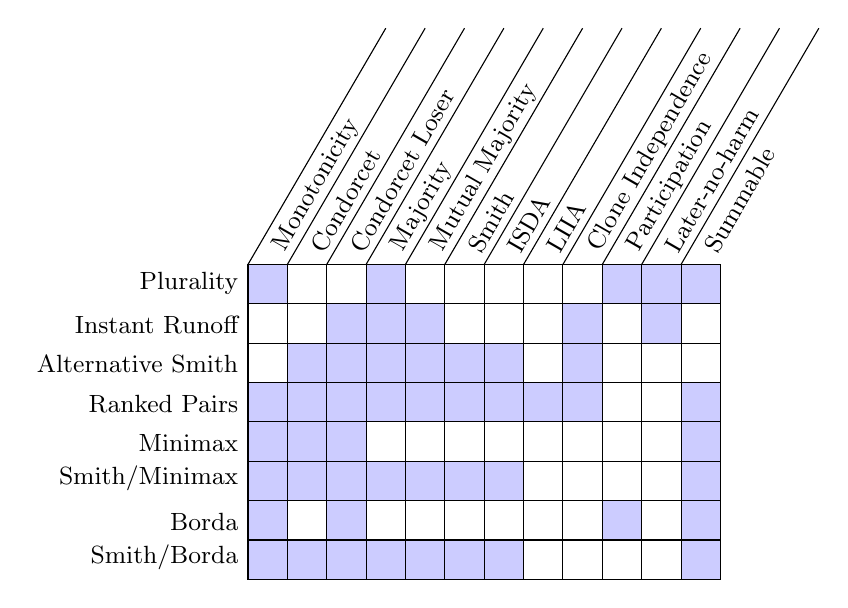
\begin{tikzpicture}[
        %sibling distance=10em,
        font=\small,
        ]
%        \foreach \x / \y in {
%            0/2,
%            1/3,
%            2/3,
%            3/4,
%            4/4,
%            5/5,
%            6/6,
%            7/7,
%            8/4,
%            9/7
%        }
%        {
%            \draw [fill=green] (\x/2,1-\y/2) rectangle ++(0.5,-0.5);
%        }
        \foreach \x / \y in {
            0/0, 3/0, 9/0, 10/0, 11/0, % Plurality
            2/1, 3/1, 4/1, 8/1, 10/1, % IRV
            1/2, 2/2, 3/2, 4/2, 5/2, 6/2, 8/2, % Alternative Smith
            0/3, 1/3, 2/3, 3/3, 4/3, 5/3, 6/3, 7/3, 8/3, 11/3, % Ranked Pairs
            0/4, 1/4, 2/4, 11/4, % Minimax
            0/5, 1/5, 2/5, 3/5, 4/5, 5/5, 6/5, 11/5, % Smith/Minimax
            0/6, 2/6, 9/6, 11/6, % Borda
            0/7, 1/7, 2/7, 3/7, 4/7, 5/7, 6/7, 11/7 % Smith/Borda
        }
        {
            \draw [fill=blue!20] (\x/2,0-\y/2) rectangle ++(0.5,-0.5);
        }
        \foreach \x[count=\xi] in {
            Monotonicity,
            Condorcet,
            Condorcet Loser,
            Majority,
            Mutual Majority,
            Smith,
            ISDA,
            LIIA,
            Clone Independence,
            Participation,
            Later-no-harm,
            Summable
        }
        {
            \node at (0.5*\xi-0.35,0) [anchor=south west] {\rotatebox{60}{\x}};
            \draw (0.5*\xi-0.5,0) -- ++(1.75,3);
            \draw (0.5*\xi-0.5,0) -- ++(0,-9/2+0.5);
        }

        \draw (0,0) -| ++(6,-4);
        \foreach \x[count=\xi] in {
            Plurality,
            Instant Runoff,
            Alternative Smith,
            Ranked Pairs,
            Minimax,
            {Smith/Minimax},
            Borda,
            Smith/Borda
        }
        {
            \node at (0,-0.5*\xi) [anchor=south east] {\x};
            \draw (0,-0.5*\xi) -- (6,-0.5*\xi);
        }

    \end{tikzpicture}
    \caption{\label{fig:single-winner-criteria}Single-winner voting rule criteria.}
\end{figure}